\chapter{Wstęp}

\section{Cel zajęć}

Celem zajęć było przygotowanie sterownika dla modelu helikoptera znajdującego się w laboratorium, którego uproszczony schemat przedstawiono na rysunku \ref{heli_model}. Jako środowisko programowe wykorzystano aplikację MATLAB wraz z pakietem Simulink. Wykorzystanie tych narzędzi polegało na komunikacji z rzeczywistym modelem helikoptera oraz wykonaniu modelu symulacyjnego.

\section{Obiekt sterowania}

Obiektem sterowania był model helikoptera o dwóch osiach swobody, który posiadał dwa wejścia (sterowanie silnikami, które napędzały śmigła) oraz dwa wyjścia (prędkość śmigła mierzona przez tachoprądnicę oraz położenie belki odczytywane z enkodera).


\begin{figure}[h!]
	\centering
	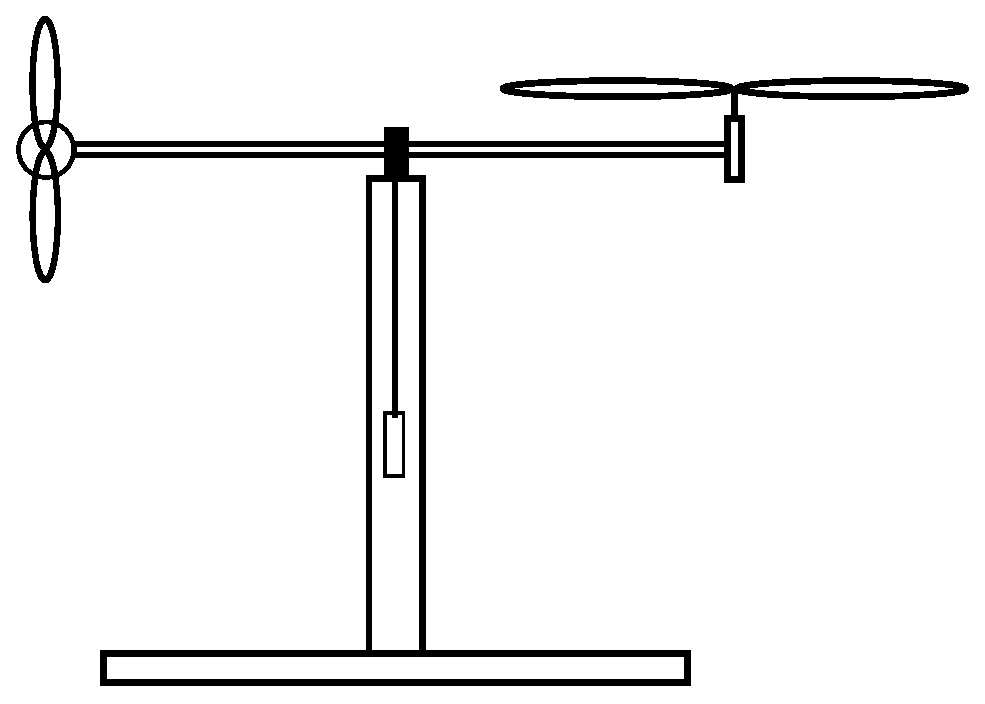
\includegraphics[scale = 0.6]{fig/model_helikoptera.eps}
	\caption		
	{Helikopter - schemat obiektu sterowania}
	\label{heli_model}
\end{figure} 

Na laboratorium zaimplementowano sterownik którego zadaniem było takie manipulowanie prędkościami silników helikoptera, aby ustabilizować obiekt w wybranym punkcie pracy. 

\section{Środowisko programowe}

Do implementacji sterownika wykorzystano środowisko programistyczne MATLAB/Simulink, w którego skład wchodziła biblioteka odpowiedzialna za komunikację z kartą RT-DAC4/PCI. Narzędzie to wykorzystano nie tylko do stworzenia panelu operacyjnego ale również do implementacji regulatorów, optymalizacji modelu i doboru odpowiednich nastaw. Panel operacyjny sterownika przedstawiono na rysunku \ref{heli_panel}.  

\begin{figure}[h!]
	\centering
	\includegraphics[scale = 1]{fig/heli_panel.png}
	\caption		
	{Panel operacyjny sterownika}
	\label{heli_panel}
\end{figure}